% CS631 Advanced Programming in the UNIX Environment
% Author: Jan Schaumann <jschauma@netmeister.org>

\documentclass[xga]{xdvislides}
\usepackage[landscape]{geometry}
\usepackage{graphics}
\usepackage{graphicx}
\usepackage{colordvi}

\begin{document}
\setfontphv

%%% Headers and footers
\lhead{\slidetitle}
\chead{CS631 - Advanced Programming in the UNIX Environment}
\rhead{Slide \thepage}
\lfoot{\Gray{Lecture 08: Interprocess Communication I}}
\cfoot{\relax}
\rfoot{\Gray{\today}}

\vspace*{\fill}
\begin{center}
	\Hugesize
		CS631 - Advanced Programming in the UNIX Environment\\
		%\vspace{.1in}\includegraphics[scale=0.5]{pics/j1.eps} \\
		Interprocess Communication I\\
	\hspace*{5mm}\blueline\\ [1em]

	\Normalsize
		Department of Computer Science\\
		Stevens Institute of Technology\\
		Jan Schaumann\\
		\verb+jschauma@cs.stevens.edu+\\
		\verb+https://stevens.netmeister.org/631/+
\end{center}
\vspace*{\fill}

\subsection{System V IPC}
Three types of {\em asynchronous} IPC originating from System V:
\begin{itemize}
	\item Semaphores
	\item Shared Memory
	\item Message Queues
\end{itemize}
\vspace{.5in}

All three use {\em IPC structures}, referred to by an {\em identifier} and a
{\em key}; all three are (necessarily) limited to communication between
processes on one and the same host.
\\

Since these structures are not known by name, special system calls ({\tt
msgget(2)}, {\tt semop(2)}, {\tt shmat(2)}, etc.) and special userland
commands ({\tt ipcrm(1)}, {\tt ipcs(1)}, etc.) are necessary.


\subsection{System V IPC: Semaphores}
A semaphore is a counter used to provide access to a shared data object for
multiple processes.  To obtain a shared resource a process needs to do the
following: \\

\begin{enumerate}
	\item Test semaphore that controls the resource.
	\item If value of semaphore $>$ 0, decrement semaphore and use resource;
		increment semaphore when done
	\item If value == 0 sleep until value $>$ 0
\end{enumerate}
\vspace{.5in}
Semaphores are obtained using {\tt semget(2)}, properties controlled using
{\tt semctl(2)}, operations on a semaphore performed using {\tt semop(2)}.

\subsection{System V IPC: Semaphores}
\begin{verbatim}
$ cc -Wall semdemo.c
1$ ./a.out

2$ ./a.out

$ ipcs -s

$ ipcrm -s 1234

1$ ./a.out
^Z

2$ ./a.out

\end{verbatim}

\subsection{IPC data flow}
\begin{center}
	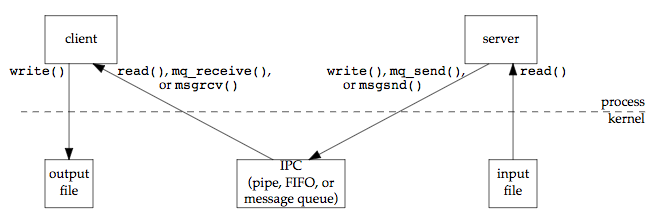
\includegraphics[angle=-90,scale=0.8]{pics/ipcflow.eps}
\end{center}

\subsection{System V IPC: Shared Memory}

\begin{center}
	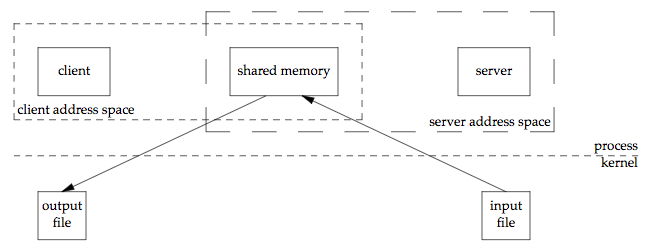
\includegraphics[angle=-90,scale=0.8]{pics/shmflow.eps}
\end{center}



\subsection{System V IPC: Shared Memory}
\begin{itemize}
	\item fastest form of IPC
	\item access to shared region of memory often controlled using
		semaphores
	\item obtain a shared memory identifier using {\tt shmget(2)}
	\item catchall for shared memory operations: {\tt shmctl(2)}
	\item attach shared memory segment to a processes address space by
		calling {\tt shmat(2)}
	\item detach it using {\tt shmdt(2)}
\end{itemize}

\subsection{System V IPC: Shared Memory}
\begin{verbatim}
$ cc -Wall shmdemo.c
$ ./a.out "Cow says: 'Moo!'"
$ ./a.out
$ ipcs -m
\end{verbatim}

\subsection{System V IPC: Shared Memory}
\begin{verbatim}
$ cc -Wall memory-layout.c
$ ./a.out
array[] from 804a080 to 8053cc0
stack around bffff9e4
malloced from 8053cc8 to 806c368
shared memory attached from 40162000 to 4017a6a0
\end{verbatim}
\begin{center}
	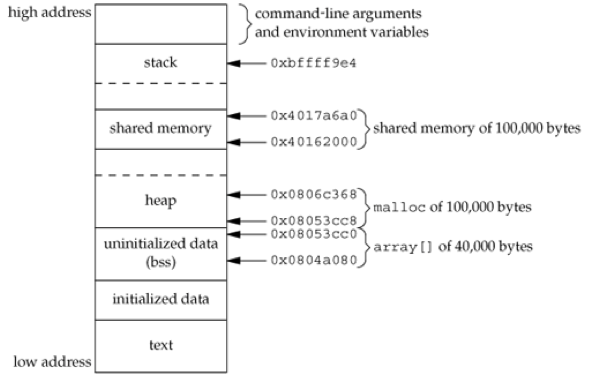
\includegraphics[angle=-90,scale=0.5]{pics/memory-layout.eps}
\end{center}

\subsection{System V IPC: Message Queues}
\begin{itemize}
	\item linked list of messages stored in the kernel
	\item create or open existing queue using {\tt msgget(2)}
	\item add message at end of queue using {\tt msgsnd(2)}
	\item control queue properties using {\tt msgctl(2)}
	\item receive messages from queue using {\tt msgrcv(2)}
\end{itemize}
\vspace{.5in}
The message itself is contained in a user-defined structure such as
\begin{verbatim}
     struct mymsg {
         long mtype;      /* message type */
         char mtext[512]; /* body of message */
     };
\end{verbatim}

\subsection{System V IPC: Message Queues}
\begin{verbatim}
$ cc -Wall msgsend.c -o msgsend
$ cc -Wall msgrecv.c -o msgrecv
$ ipcs -qo
$ ./msgsend 1 'Hello!'
$ ipcs -qo
$ ./msgsend 1 'How are you?'
$ ipcs -qo
$ ./msgrecv 1
$ ipcs -qo
$ ./msgrecv 1
$ ipcs -qo
$ ./msgrecv 1
^C
$ ipcs -q
$ ./msgsend 2
$ ipcrm -q <msqid>
\end{verbatim}

\subsection{POSIX Message Queues}
{\tt mq(3)} provides an real-time IPC interface
similar to System V message queues.  Notably:

\begin{itemize}
	\item message queues are identified by a named
identifier (no {\tt ftok(3)} needed); may or may not
be exposed in the file system (e.g. {\tt /dev/mqueue})
	\item {\tt mq\_send(3)} and {\tt
mq\_receive(3)} allow both blocking and non-blocking
calls
	\item {\tt
mq\_send(3)} lets you specify a priority; equal
priority messages are queued as a FIFO, but higher
priority messages are inserted before those of a lower
priority
	\item {\tt mq(3)} provides an asynchronous
notification mechanism: {\tt mq\_notify(3)}
\end{itemize}

\subsection{POSIX Message Queues}
\begin{verbatim}
$ cc $CFLAGS mqrecv.c -o mqrecv -lrt
$ cc $CFLAGS -DWAIT mqsend.c -o mqsend
$ ./mqrecv

$ ./mqsend bacon avocado

$ ./mqrecv wait

$ ./mqsend bacon avocado

$ cc $CFLAGS mqsend.c -o mqsend

$ ./mqsend bacon avocado
\end{verbatim}

\subsection{Pipes: {\tt pipe(2)}}
\small
\setlength{\unitlength}{1mm}
\begin{center}
	\begin{picture}(150,22)
		\thinlines
		\put(0,0){\framebox(130,22){}}
		\put(10,17){{\tt \#include <unistd.h>}}
		\put(10,10){{\tt int pipe(int {\em filedes[2]});}}
		\put(80,3){Returns: 0 if OK, -1 otherwise}
	\end{picture}
\end{center}
\Normalsize
\begin{itemize}
	\item oldest and most common form of UNIX IPC
	\item half-duplex (on some versions full-duplex)
\end{itemize}

\subsection{Pipes: {\tt pipe(2)}}
\begin{center}
	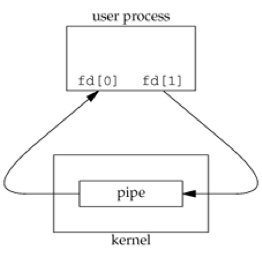
\includegraphics[angle=-90,scale=0.8]{pics/pipe1.eps}
\end{center}

\subsection{Pipes: {\tt pipe(2)}}
\begin{center}
	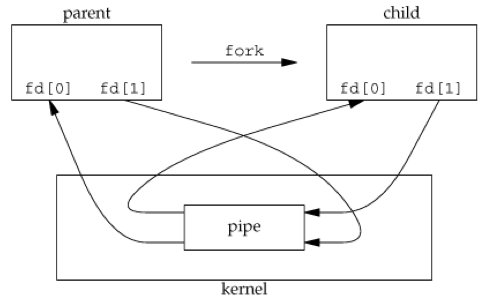
\includegraphics[angle=-90,scale=0.8]{pics/pipe2.eps}
\end{center}

\subsection{Pipes: {\tt pipe(2)}}
\begin{center}
	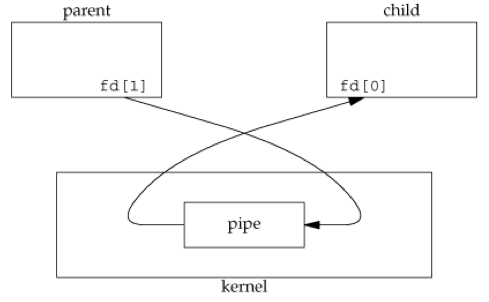
\includegraphics[angle=-90,scale=0.8]{pics/pipe3.eps}
\end{center}

\subsection{Pipes: {\tt pipe(2)}}
\begin{verbatim}
$ cc -Wall pipe1.c
$ ./a.out
P=> Parent process with pid 23988 (and its ppid 7474).
P=> Sending a message to the child process (pid 23989):
C=> Child process with pid 23989 (and its ppid 23988).
C=> Reading a message from the parent (pid 23988):
Hello child!  I'm your parent pid 23988!
$
\end{verbatim}
\vfill
%\hfill \includegraphics[scale=0.9]{pics/j2.eps}


\subsection{Pipes: {\tt pipe(2)}}
\begin{verbatim}
$ cc -Wall pipe1.c
$ ./a.out
P=> Parent process with pid 23984 (and its ppid 7474).
P=> Sending a message to the child process (pid 23985):
C=> Child process with pid 23985 (and its ppid 1).
C=> Reading a message from the parent (pid 1):
Hello child!  I'm your parent pid 23984!
$
\end{verbatim}
\vfill

\subsection{Pipes: {\tt pipe(2)}}
\begin{verbatim}
$ cc -Wall pipe1.c
$ ./a.out
P=> Parent process with pid 23986 (and its ppid 7474).
P=> Sending a message to the child process (pid 23987):
C=> Child process with pid 23987 (and its ppid 23986).
C=> Reading a message from the parent (pid 1):
Hello child!  I'm your parent pid 23986!
$
\end{verbatim}
\vfill

\subsection{Pipes: {\tt pipe(2)}}
A more useful example: displaying some content using the user's preferred
pager.  (Look, Ma, no temporary files!)
\begin{verbatim}
$ cat pipe2.c | ${PAGER:-/usr/bin/more}
$ cc -Wall pipe2.c
$ echo $PAGER

$ ./a.out pipe2.c
[...]
^Z
$ ps -o pid,ppid,comm
  PID  PPID COMMAND
22306 26650 ./a.out pipe2.c
22307 22306 more
23198 26650 ps -o pid,ppid,comm
26650 26641 -ksh
$ fg
$ env PAGER=/bin/cat ./a.out pipe2.c
\end{verbatim}


\subsection{Pipes: {\tt pipe(2)}}
\small
\setlength{\unitlength}{1mm}
\begin{center}
	\begin{picture}(150,22)
		\thinlines
		\put(0,0){\framebox(130,22){}}
		\put(10,17){{\tt \#include <unistd.h>}}
		\put(10,10){{\tt int pipe(int {\em filedes[2]});}}
		\put(80,3){Returns: 0 if OK, -1 otherwise}
	\end{picture}
\end{center}
\Normalsize
\begin{itemize}
	\item oldest and most common form of UNIX IPC
	\item half-duplex (on some versions full-duplex)
	\item can only be used between processes that have a common ancestor
	\item can have multiple readers/writers ({\tt PIPE\_BUF} bytes are
		guaranteed to not be interleaved)
\end{itemize}
\vspace{.5in}

Behavior after closing one end:
\begin{itemize}
	\item {\tt read(2)} from a pipe whose write end has been closed returns 0
		after all data has been read
	\item {\tt write(2)} to a pipe whose read end has been closed generates
		{\tt SIGPIPE} signal.  If caught or ignored, {\tt write(2)} returns an
		error and sets {\tt errno} to {\tt EPIPE}.
\end{itemize}

\subsection{Pipes: {\tt popen(3)} and {\tt pclose(3)}}
\small
\setlength{\unitlength}{1mm}
\begin{center}
	\begin{picture}(150,40)
		\thinlines
		\put(0,0){\framebox(130,40){}}
		\put(10,35){{\tt \#include <stdio.h>}}
		\put(10,28){{\tt FILE *popen(const char *{\em cmd}, const char *{\em type});}}
		\put(62,21){Returns: file pointer if OK, {\tt NULL} otherwise}
		\put(10,10){{\tt int pclose(FILE *{\em fp});}}
		\put(55,3){Returns: termination status {\em cmd} or -1 on error}
	\end{picture}
\end{center}
\Normalsize
\vspace{.5in}
\begin{itemize}
	\item historically implemented using unidirectional pipe (nowadays
		frequently implemented using sockets or full-duplex pipes)
	\item {\em type} one of ``r'' or ``w'' (or ``r+'' for
		bi-directional communication, if available)
	\item {\em cmd} passed to {\tt /bin/sh -c}
\end{itemize}

\subsection{Pipes: {\tt popen(3)} and {\tt pclose(3)}}
\begin{verbatim}
$ cc -Wall popen.c
$ echo $PAGER

$ ./a.out popen.c
[...]
$ env PAGER=/bin/cat ./a.out popen.c
[...]
$
\end{verbatim}
\vfill
%\hfill \includegraphics[angle=-90,scale=0.9]{pics/j3.eps}

\subsection{Pipes: {\tt popen(3)} and {\tt pclose(3)}}
\begin{verbatim}
$ cc -Wall popen.c
$ echo $PAGER

$ ./a.out popen.c
[...]
$ env PAGER=/bin/cat ./a.out popen.c
[...]
$ env PAGER=/bin/cat/foo ./a.out popen.c
sh: /bin/cat/foo: Not a directory
$ env PAGER="more; touch /tmp/boo" ./a.out popen.c
$ env PAGER="more; rm /etc/passwd 2>/dev/null" ./a.out popen.c
\end{verbatim}
\vfill
%\hfill \includegraphics[scale=0.9]{pics/j4.eps}


\subsection{FIFOs: {\tt mkfifo(2)}}
\small
\setlength{\unitlength}{1mm}
\begin{center}
	\begin{picture}(150,22)
		\thinlines
		\put(0,0){\framebox(130,22){}}
		\put(10,17){{\tt \#include <sys/stat.h>}}
		\put(10,10){{\tt int mkfifo(const char *{\em path}, mode\_t {\em mode});}}
		\put(80,3){Returns: 0 if OK, -1 otherwise}
	\end{picture}
\end{center}
\Normalsize

\begin{itemize}
	\item aka ``named pipes''
	\item allows unrelated processes to communicate
	\item just a type of file -- test for using {\tt S\_ISFIFO(st\_mode)}
	\item {\em mode} same as for {\tt open(2)}
	\item use regular I/O operations (ie {\tt open(2)}, {\tt read(2)}, {\tt
		write(2)}, {\tt unlink(2)} etc.)
	\item used by shell commands to pass data from one shell
			pipeline to another without creating intermediate
			temporary files
\end{itemize}

\subsection{FIFOs: {\tt mkfifo(2)}}
Example: split input into sets
\begin{center}
	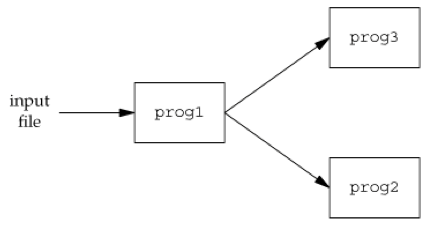
\includegraphics[angle=-90,scale=0.8]{pics/fifo1.eps}
\end{center}

\subsection{FIFOs: {\tt mkfifo(2)}}
Example: split input into sets
\begin{center}
	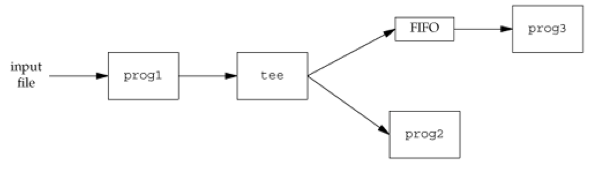
\includegraphics[angle=-90,scale=0.8]{pics/fifo2.eps}
\end{center}
\begin{verbatim}
$ mkfifo fifo
$ grep pattern fifo > match &
$ gzcat file.gz | tee fifo | grep -v pattern > nomatch
\end{verbatim}
\vfill
%\hfill \includegraphics[scale=0.9]{pics/j5.eps}

\subsection{In-class coding exercise}
Implement the 'command' function: \\

\vspace{1in}
\verb+https://stevens.netmeister.org/631/f18-hw2.html+

\subsection{Reading}
\begin{itemize}
	\item \verb+https://stevens.netmeister.org/631/ipctut.pdf+
	\item \verb+https://stevens.netmeister.org/ipc.pdf+
	\item \verb+https://beej.us/guide/bgipc/html/single/bgipc.html+
	\item \verb+https://is.gd/M2dkju+
\end{itemize}

\end{document}
